\documentclass[a4paper, 12pt]{article}
\usepackage[ngerman]{babel}
\usepackage[utf8]{inputenc}
\usepackage[T1]{fontenc}
\usepackage{fontspec}
\usepackage{amssymb}
\usepackage{xcolor}
\usepackage{tikz}
\usepackage{tabularx}
\usepackage{enumitem}
\usepackage{listings}
\usepackage{graphicx}
\usepackage{hyperref}
\usepackage[top=2.5cm, bottom=2cm, left=2cm, right=2cm]{geometry}
\usepackage{fancyhdr}

% header style
\pagestyle{fancy}
\fancyhf{}
\rhead{\thepage}
\lhead{\textit{SW-Projekt 2021/22}}
\chead{\textit{ViViPlayer3}}

% pdf options
\hypersetup{
	pdfauthor = {Gruppe ViViPlayer3},
	pdftitle = {Spezifikation ViViPlayer3},
	pdfsubject = {Softwareprojekt},
	pdfcreator = {VORNAME NACHNAME}}

% command to add the signateure-fields
\newcommand*{\SignatureAndDate}[1]{%
    \par\noindent\makebox[\linewidth]{\hrulefill}%
    \par\noindent\makebox[\linewidth][l]{#1}%
}%

% command to add a TODO Line
\newcommand*{\todo}[1]{\textbf{\textcolor{red}{TODO: #1}\\}}

\definecolor{lightlightgray}{RGB}{222,222,222}

\begin{document}
	\thispagestyle{empty} % no header on first page
	\begin{center}
		{\Huge Softwareprojekt Wintersemester 2021/2022}\\[.35cm]
		{\large am Fachgebiet Software Engineering, Leibniz Universität Hannover}\\[.1cm]
	\end{center}
	\begin{center}
	\colorbox{lightlightgray}{
		\begin{minipage}{\linewidth}
			\begin{center}
				\vspace{0.2cm}
				{\Huge Spezifikation}\\[.1cm]
				{\Huge ViViPlayer3}\\[.3cm]
				\texttt{SWP-WS2122-ViViPlayer3-Spec-v01.pdf}
				\vspace{0.2cm}
			\end{center}
		\end{minipage}
	}
	\end{center}
	\textbf{Vorgelegt}\\
		\hspace*{1cm}am 14.11.2021 \\
		\hspace*{1cm}von ViViPlayer3\\[0.2cm]
	\textbf{Ausführende:}
		\begin{center}
			\begin{tabular}{|l|l|l|}
				\hline
				\textit{Nachname} 				& \textit{Vorname} 	& \textit{Rolle} \\ \hline\hline
				Nguyen							& Dinh Minh			& Projektleiter \\ \hline
				Anfuso							& Matthew			& Qualitätsbeauftragter \\ \hline
				Bohlmann						& Tim				& Entwickler \\ \hline
				Tran							& The				& Entwickler \\ \hline
				Hartmann						& Jakob				& Entwickler \\ \hline
				Puglisi							& Joshua			& Entwickler \\ \hline
			\end{tabular}
		\end{center}
		\vspace{0.3cm}
	\textbf{Das Dokument enthält}\\[0.1cm]
		\hspace*{1cm}$\boxtimes$ Die Anforderungen aus Kundensicht (User Requirements)\\[0.1cm]
		\hspace*{1cm}$\boxtimes$ Anforderungen, wie das zu System zu gestalten ist (System Requirements)\\[1cm]
	\SignatureAndDate{Datum, Unterschrift des Projektleiters, auch für die anderen Projektangehörigen}\\[0.3cm]
	\textbf{Kunden-Bewertung}\\[0.4cm]
		Der Kunde, Jianwei Shi, bestätigt mit seiner Unterschrift, diese Anforderungsspezifikation erhalten, geprüft und für inhaltlich $\square$ \textbf{in Ordnung} \textbar~ $\square$ \textbf{weitgehend in Ordnung} \textbar ~ $\square$ \textbf{deutlich zu verbessernd} \textbar ~ $\square$ \textbf{nicht akzeptabel} befunden zu haben.\\[1cm]
	\SignatureAndDate{Datum, Unterschrift des Kunden; evtl. Vermerk.}

	\pagebreak
	\tableofcontents
	\pagebreak

	\raggedright

	\section{Mission des Projekts}

\subsection{Erläuterung des zu lösenden Problems}
Das Projekt ViViPlayer (Visionsvideo Player) ist eine Webanwendung, welche die gemeinsame Arbeit 
bei der Anforderungsanalyse im Requirement Engineering effektiver und kommunikativer macht.
Es ist möglich sich gemeinsam ein Visionsvideo anzuschauen und direkt in der Anwendung User Stories
zu verfassen. Durch interaktive Funktionen kann man sich einen Überblick schaffen über die Ansichten und Vorstellungen der Teilnehmer.

Die Anwendung verfolgt also das Ziel die effektiv Anforderungen zu sammeln und dabei alle möglichst viel mit einzubeziehen.
Deswegen ist dieses Projekt als Webanwendung konzipiert, um möglichst vielen einfachen Zugriff auf das Programm zu geben.

\subsection{Wünsche und Prioritäten des Kunden}
	Es folgen die Wünsche des Kunden, nach absteigender Priorität geordnet:
	\begin{itemize}
		\item In der Webanwendung ist es möglich synchron mit den anderen Teilnehmern Video wiederzugeben. Der Moderator ist hierbei derjenige der den Player bedient.
		\item Der Moderator kann entweder das Video bis zum Ende abspielen oder bis zum nächsten Segment.
		\item Das Video wird automatisch segmentiert, sodass der Moderator an die verschiedenen Punkte springen kann. Der Moderator kann manuell segmentieren.
		\item Die Teilnehmer können User Stories zu einer Einstellung oder mehreren Einstellungen direkt in der Webanwendung erstellen mit Hilfe einer Schablone.
		\item Die Teilnehmer können sich vertraulich und sicher mit einem Passwort anmelden.
		\item User Stories können direkt zu dem JIRA Board exportiert werden. Man kann diese User Stories direkt integrieren.
		\item Es ist möglich direkt Verständnisfragen zu stellen.
		\item Annotationen können direkt im Video eingeblendet werden.
		\item Die Screenshots zu den verschiedenen Segmenten im Video können in eine .odt exportiert werden.
		\item Implementierung anhand von Design Patterns zur späteren Erweiterung als Android App zum Beispiel.
		\item Die Webanwendung kann automatisch vervollständigen oder Rückmeldungen anhand von Anleitungen.
	\end{itemize}

\subsection{Domänenbeschreibung}
    Eingesetzt wird dieses Programm in einem Treffen mit einem Kunden zur Anforderungsanalyse.
    Hierbei kann sich sowohl Online als auch in Präsenz getroffen werden. Auch eine hybride Variante,
    wo sowohl Online- als auch Präsenzteilnehmer anwesend sind ist denkbar. 
    Anwesend sind immer ein bis zwei Moderatoren, die die Sitzung leiten und den Videoplayer bedienen.
	Zielgruppe sind also sowohl die Entwickler als auch der Vertreter des Kundens, welcher auch verantwortlich für die Anforderungen ist.
\subsection{Maßnahmen zur Anforderungsanalyse}
    Um die Anforderungen auf unserer Seite zu klären haben wir mehrere Prototypen gebaut.
    Direkt zu Anfang haben wir einen Prototypen erstellt, um zu ermitteln wie man Video segmentieren kann.
    Zudem haben wir einen weiteren Prototypen erstellt, mit welchem wir die Synchronisation erprobt haben.
    Hierbei stand rein die technische Umsetzung im Vordergrund und wie man Videos synchronisieren kann.
    Beide Prototypen sind JavaScript Anwendungen die bereits im Browser laufen.   
	\pagebreak
	\section{Rahmenbedingungen und Umfeld}

\subsection{Einschränkungen und Vorgaben}
Der Zugang zu der Web-App ist durch Anmeldedaten beschränkt, d.h. sind Username und Passwort notwendig, um sich einzuloggen. Alternative Login wie TAN ist auch möglich. Nutzer kann entweder als Moderator einloggen oder als Teilnehmer. Moderator und Teilnehmer können in dieser Web-App gleichzeitig eine interaktive Informationsaustausch durchführen, also eine Session. Eine Session kann allerdings nur von dem Moderator vorbereitet werden.\linebreak
\linebreak
Bevor ein Session anfängt, hat der Moderator die Möglichkeiten, Video von Cloud einzubetten, das Video abzuspielen und auch zu segmentieren. Nachdem Hochladen konnte der Moderator das Video entweder automatisch oder manuell segmentieren. Noch ein weiteres Feature ist Annotationen für Verständnisfragen in dem Video zu legen. Werden keine weitere Änderungen für das Video gemacht, kann Moderator auf ''Fertig'' klicken, dann startet eine Session.\linebreak
\linebreak
Während des Sessions kann der Moderator das Video abspielen und navigieren für den Teilnehmer. Teilnehmer kann das Abspielen des Videos live verfolgen, Fragen beantworten, und auch Stories schreiben. Würde eine Frage im bestimmten Zeitpunkt kommen, kann der Teilnehmer auf die Antwort einfach klicken, und die wird dann gleich in Form eines Balken- oder Kreisdiagramms sichtbar. Der Teilnehmer kann auch eine alternative Antwortmethode wählen, falls eine Umfrage nicht bevorzugt wird. Alle Annotationen und Antworten werden als odt-Datei zusammengefasst, und im Server gespeichert. Zum Schreiben der User Stories kann auch der Teilnehmer ein Screenshot hinfügen mit Copy und Paste. Schlusselsätze als odt-Datei zusammen mit dem Screenshot werden zu JIRA Board exportiert.\linebreak
\linebreak
Nach Kundenpräferenz ist die Anzahl von Moderator und Teilnehmer 18 Personen in einem Session.

\subsection{Anwender}
Die Web-App ist für Softwareentwickler und auch Kunden, die Kenntnise über Requirements Engineering besetzen, geeignet. Was gemeint hier bei Kunden ist, diejenigen, den das Projekt gehört. In einem Session wird Softwareentwickler Moderator, und die Kunden werden Teilnehmer sein. Die Web-App sollte von Nutzer mit durchschnittlichen Computerkenntnisse bedienbar sein, damit sie sich leicht durch die Web-App navigieren lassen.

\subsection{Schnittstellen und angrenzende Systeme} 
In diesem Projekt wird Django als Framework benutzt, da Django sowohl Frontend als auch Backend übernimmt. HTML5, CSS, JavaScript können in Django integriert werden mithilfe von frontend Bibliotheken von Django. Für Backend wird SQLite als Datenbank benutzt.
	\pagebreak
	\section{Funktionale Anforderungen}

\subsection{Use Case-Diagramm}
\begin{figure}[h!]
	\centering
	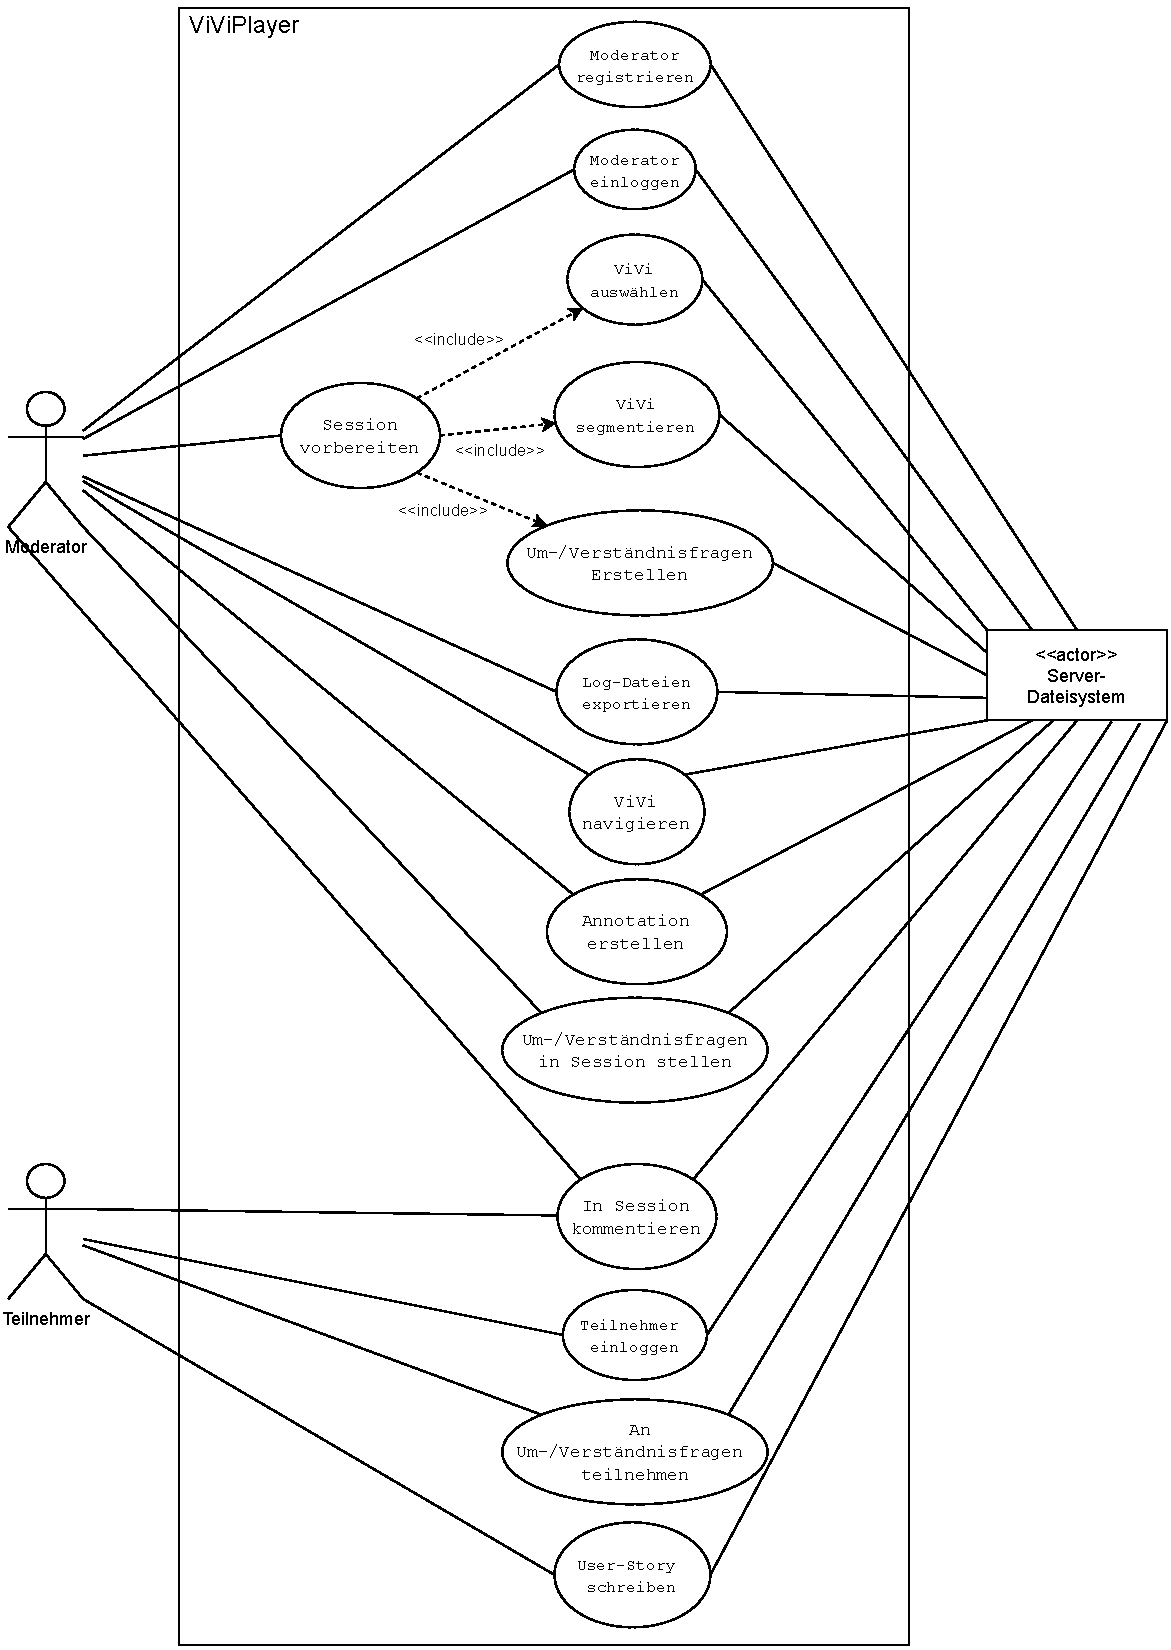
\includegraphics[width=0.9545\textwidth]{sections/diagrams/viviplyer-uc-diagramm.pdf}
\end{figure}
\pagebreak

\subsection{Use Case-Beschreibungen}

\subsubsection{UC: Moderator registrieren}
\begin{tabularx}{\linewidth}{|l|X|}
	\hline
	Use Case Nr. 01			& \textbf{Moderator registrieren} \\ \hline
	Erläuterungen			& Um alle Rechte eines Moderators zu bekommen, muss ein 
							Benutzer als Moderator registriert werden. \\ \hline
	Systemgrenzen (Scope)	& Registrierung-System. \\ \hline
	Ebene					& Hauptfunktion \\ \hline
	Vorbedingung			& Die Web-App ist betriebsbereit. Der Benutzer befindet sich auf die 
							  Hauptseite von ViViPlayer-Web-App. \\ \hline
	Mindestgarantie			& Im Fehlerfall wird kein neues Moderator-Konto im System 
	                          registriert. Klare Fehlermeldung wird ausgegeben. \\ \hline
	Erfolgsfall  			& Ein neues Moderator-Konto wurde erstellt. \\ \hline
	Stakeholder				& Systembediener (Moderator) - möchte die Funktionen der Web-App so 
							  schnell wie möglich nutzen. \\
							& Systembesitzer (Systemadministrator) - möchte, dass die Funktionen 
							  der Web-App für die Benutzer mit korrekten Zugriffsrechten verfügbar sind.\\ \hline
	Hauptakteur				& Systembediener (Moderator) \\ \hline
	Auslöser				& Der Benutzer klickt auf den ``Registrieren''-Button. \\ \hline	
	Hauptszenario			& 1. Der Benutzer klickt auf den ``Registrieren''-Button. \\
							& 2. Das System fordert den Benutzer auf, eine Email-Adresse 
							  sowie die Passwort für das neue Konto einzugeben. \\
							& 3. Der Benutzer gibt seinen Benutzername und seine Passwort 
							  ein und bestätigt sie \\
							& 4. Das System und ein anderer Moderator validiert die vom 
							  Benutzer eingegebene Daten. Eine Meldung wird als 
							  Anleitung angezeigt, was der neue Benutzer weiter machen soll. \\
							& 5. Der Benutzer wird zurück zur Hauptseite geleitet. 
							  \\ \hline
	Erweiterungen			& 4a. WENN das System feststellt, dass die eingegebene Daten 
							  (Benutzername und Passwort) nicht gültig sind, DANN wird eine Fehlermeldung ausgegeben. Zurück zu Schritt 2. \\ \hline
	Priorität				& niedrig \\ \hline
	Verwendungshäufigkeit	& weniger häufig \\ \hline
\end{tabularx}

\pagebreak

\subsubsection{UC: Moderator einloggen}
\begin{tabularx}{\linewidth}{|l|X|}
	\hline
	Use Case Nr. 02			& \textbf{Moderator einloggen} \\ \hline
	Erläuterungen			& Der Benutzer möchte sich als Moderator einloggen, damit er eine 
							  Session im ViViPlayer abhalten kann. \\ \hline
	Systemgrenzen (Scope)	& Login-System \\ \hline
	Ebene					& Hauptfunktion \\ \hline
	Vorbedingung			& Die Web-App ist betriebsbereit. Der Benutzer befindet sich auf
							  Hauptseite der Web-App. \\ \hline
	Mindestgarantie			& Das Einloggen des Benutzers wird abgesagt, falls der eingegebene
							  Benutzername/die Email-Adresse nicht im Datenbank oder die Passwort falsch ist. Eine Fehlermeldung wird dann ausgegeben.
							  \\ \hline
	Erfolgsfall 			& Der Zugriff des Benutzers wurde erfolgreich bestätigt. Der
							  Benutzer befindet sich auf der Moderator-Hauptseite. 
							  \\ \hline
	Stakeholder				& Systembediener (Moderator) - möchte die Funktionen der Web-App 
							  schnell wie möglich nutzen. \\
							& Systembesitzer (Systemadministrator) - möchte, dass die Funktionen 
							  der Web-App für die Benutzer mit korrektem Zugriffsrecht verfügbar sind.\\ \hline
	Hauptakteur				& Systembediener (Moderator) \\ \hline
	Auslöser				& Der Benutzer klickt auf die ``Einloggen als Moderator''-Option.\\ 
							  \hline	
	Hauptszenario			& 1. Der Benutzer klickt auf die ``Einloggen als 
							  Moderator''-Option.\\
							& 2. Das System zeigt das Moderator-Loginsformular an. \\
							& 3. Der Benutzer gibt sein Benutzername/seine Email-Adresse und 
							  seine Passwort ein. \\
							& 4. Das System validiert die vom Benutzer eingegebene
							  Log-in-Daten. \\
							& 5. Der Benutzer wird im System angemeldet und weiter zur
							  Moderator-Hauptseite geleitet. \\ \hline
	Erweiterungen			& 1a. WENN das System feststellt, dass die eingegebene Daten 
							  (Benutzername/Email-Adresse und Passwort) nicht abgestimmt sind, DANN wird eine Fehlermeldung ausgegeben. Zurück zu Schritt 2. \\ \hline
	Priorität				& mittel \\ \hline
	Verwendungshäufigkeit	& häufig \\ \hline
\end{tabularx}

\pagebreak

\subsubsection{UC: Teilnehmer einloggen}
\begin{tabularx}{\linewidth}{|l|X|}
	\hline
	Use Case Nr. 03			& \textbf{Teilnehmer Einloggen} \\ \hline
	Erläuterungen			& Damit ein Teilnehmer alle Funktionen der App benutzen kann, 
							  muss er sein Zugriffsrecht via TAN bestätigen. \\ \hline
	Systemgrenzen (Scope)	& Login-System \\ \hline
	Ebene					& Hauptebene \\ \hline
	Vorbedingung			& Die Web-App ist betriebsbereit. Der Benutzer befindet sich in
							  Hauptseite der Web-App \\ \hline
	Mindestgarantie			& Das Log-in des Benutzers wird abgesagt, falls die eingegebene
							  TAN nicht richtig ist. Eine Fehlermeldung wird ausgegeben
							  \\ \hline
	Erfolgsfall 			& Der Zugriff des Benutzers wurde erfolgreich bestätigt. Der
							  Benutzer hat sich auf der Moderator-Hauptseite befindet. \\ \hline
	Stakeholder				& Systembediener - möchte die Funktionen der Web-App schnell 
							  wie möglich nutzen. \\
							& Herr Jianwei Shi (Systembesitzer) - möchte die Funktionen der 
							  Web-App für die Benutzer mit korrektem Zugriffsrecht verfügbar sein.\\ \hline
	Hauptakteur				& Systembediener, die Teilnehmer-Rechte haben möchten \\ \hline
	Auslöser				& Der Benutzer möchte an einem Session des ViViPlayer
							  teilnehmen. Er befindet sich auf der Hauptseite der Web-App,
							  um mit TAN einzuloggen. \\ \hline	
	Hauptszenario			& 1. Der Benutzer befindet sich auf der Hauptseite der Web-App,
	                          um mit TAN einzuloggen. \\
	                        & 2. Das System fordert den Benutzer auf, als Teilnehmer eine
							  TAN einzugeben. \\
							& 3. Der Benutzer gibt seine vom Moderator erhaltene TAN ein. \\
							& 4. Das System validiert die vom Benutzer eingegebene
							  TAN. \\
							& 5. Dem Benutzer wird im System angemeldet und weiter zur
							  Teilnehmer-Hauptseite geleitet. \\ \hline
	Erweiterungen			& 4a. Wenn das System feststellt, dass die eingegebene TAN nicht 
							  eine von System generierte TAN ist, wird eine Fehlermeldung 
							  ausgegeben. Das System geht zurück zu Schritt 2. \\ \hline
	Priorität				& mittel \\ \hline
	Verwendungshäufigkeit	& sehr häufig \\ \hline
\end{tabularx}

\pagebreak

\subsubsection{UC: Session vorbereiten}
\begin{tabularx}{\linewidth}{|l|X|}
	\hline
	Use Case Nr. 04			& \textbf{Session vorbereiten} \\ \hline
	Erläuterungen			& Bevor ein Moderator eine Session mit den Teilnehmer anfangen 
	                          kann, muss er zuerst vorbereiten. Das heißt: er muss das ViVi einbetten und segmentieren, Verständnisfragen vorbereiten und TAN für die Session erzeugen. \\ \hline
	Systemgrenzen (Scope)	& Gesamtsystem. \\ \hline
	Ebene					& Hauptfunktion. \\ \hline
	Vorbedingung			& Die Web-App ist betriebsbereit. Der Benutzer hat 
	                          Moderator-Rechte. Er wählt die Option, eine neue Session zu erstellen, von der Moderator-Hauptseite. \\ \hline
	Mindestgarantie			& Im Fehlerfall wird keine Session erstellt.\\ \hline
	Erfolgsfall  			& Das segmentierte Vision-Video sowie eine sichere TAN sind 
	                          bereitgestellt für eine ViViPlayer-Session. \\ \hline
	Stakeholder				& Systembediener (Moderator) - will eine produktive Session mit den 
	                          Teilnehmer via ViViPlayer. \\
							& Systembesitzer (Herr Jianwei Shi) - möchte, dass alle Sessions 
							  in der Web-App erfolgreich durchgeführt werden. \\ \hline
	Hauptakteur				& Systembediener (Moderator). \\ \hline
	Auslöser				& Der Benutzer klickt auf die "Session erstellen"-Option. \\ \hline	
	Hauptszenario			& 1. Der Benutzer klickt auf die "Session erstellen"-Option. \\ 
							& 2. Das System zeigt die ViVi-Auswählen-Oberfläche an. \\
							& 3. Der Benutzer wählt ein ViVi und bestätigt. (UC 5) \\ 
							& 4. Das System zeigt die ViVi-Segmentieren-Oberfläche. \\ 
							& 5. Der Benutzer segmentiert das von ihm ausgewählte Video und 
							  bestätigt. (UC 6) \\
							& 6. Das System zeigt die Frage-Vorbereiten-Oberfläche. \\
							& 7. Der Benutzer bereitet die Um-/Verstänisfragen vor und bestätigt.
							  (UC 7) \\
							& 8. Das System zeigt die ViVi-Überblick-Oberfläche. \\ 
							& 9. Der Benutzer prüft noch mal alle Vorbereitungschritte und 
							  klickt auf das "Erstellen"-Button. \\
							& 10. Das System erstellt eine neue Session und eine sichere TAN. \\ 
							  \hline
	Erweiterungen			& 4a. WENN das Video nicht eingebettet werden kann, DANN wird eine 
	                          Fehlermeldung gezeigt. Zurück zu Schritt 2. \\
							& 6a. WENN die Segmentierung nicht gültig ist, DANN wird eine 
							  Fehlermeldung ausgegeben. Zurück zu Schritt 4.\\
							& 8a. WENN es Fehler bei der Eingabe der Fragen, DANN wird 
							  eine Fehlermeldung ausgegeben. Zurück zu Schritt 4. \\ \hline
	Priorität				& hoch \\ \hline
	Verwendungshäufigkeit	& häufig \\ \hline
\end{tabularx}
\\[0.5cm]
\textbf{Erläuterungen und Details}
\begin{itemize}
	\item ViVi: die Abkürzung von dem Begriff ``Vision-Video''.
	\item ViVi-Auswählen-Oberfläche: Eine Menge von ViVis werden hier angezeigt, damit der Benutzer eines davon auswählen kann.
	\item ViVi-Segmentieren-Oberfläche: da gibt es ein Video-Fenster mit Controller, eine Liste von Segmenten mit ihrem Namen und Zeitstempeln sowie ein Button zum Hinzufügen der neuen Segmente. 
	\item Frage-Vorbereiten-Oberfläche: es gibt eine Liste von erstellten Fragen
	sowie ein Fenster zum Bearbeitung einer neuen Frage.
	\item TAN-Oberfläche: man kann entweder manuell oder automatisch TAN für die Session hier erzeugen.
	\item ViVi-Überblick-Oberfläche: hier kann der Benutzer seine schon eingegebene Konfiguration nachschauen, um Fehler zu checken.
	\item Für die ViVi-Auswählen-, ViVi-Segmentieren-, TAN- und ViVi-Überblick-Oberfläche gibt es möglich ein ``Zurück''-Button, damit man nach Wunsch modifizieren kann.
\end{itemize}
\pagebreak

\subsubsection{UC: ViVi auswählen}
\begin{tabularx}{\linewidth}{|l|X|}
	\hline
	Use Case Nr. 05			& \textbf{ViVi auswählen} \\ \hline
	Erläuterungen			& Vision-Video auswählen ist der erste Schritt zur Vorbereitung 
							  einer ViViPlayer-Session. \\ \hline
	Systemgrenzen (Scope)	& Gesamtsystem. \\ \hline
	Ebene					& Hauptebene \\ \hline
	Vorbedingung			& Die Web-App ist betriebsbereit. Der Benutzer hat 
							  Moderator-Rechte. Er wählt die Option, eine neue Session zu 
							  erstellen, auf der Moderator-Hauptseite. \\ \hline
	Mindestgarantie			& Im Fehlerfall wird kein Video ausgewählt und somit keine 
							  Session.\\ \hline
	Erfolgsfall 			& Der Benutzer konnte sein gewünschtes Video problemlos auswählen. 
							  \\ \hline
	Stakeholder				& Systembediener (Moderator) - will eine produktive Session mit den 
							  Teilnehmer via ViViPlayer. \\
							& Systembesitzer (Herr Jianwei Shi) - möchte alle Sessions in der 
							  Web-App erfolgreich durchgeführt werden. \\ \hline
	Hauptakteur				& Systembediener (Moderator). \\ \hline
	Auslöser				& Der Benutzer klickt auf die "Session erstellen"-Option. \\ \hline	
	Hauptszenario			& 1. Der Benutzer klickt auf die "Session erstellen"-Option. \\
							& 2. Das System zeigt die ViVi-Auswählen-Oberfläche an. \\
							& 3. Der Benutzer kann ein ViVi vom Server-Dateisystem auswählen 
							  und klickt auf das ``Weiter''-Button, wenn er fertig ist. \\
							& 4. Das System zeigt die ViVi-Segmentieren-Oberfläche an. \\ \hline
	Erweiterungen			& 3a. Alternativ kann das Video via Pfad eingebettet werden. \\ 
							& 4a. WENN das Video nicht ausgewählt werden kann, DANN wird eine 
							  Fehlermeldung gezeigt. Zurück zu Schritt 2. \\ \hline
	Priorität				& sehr hoch \\ \hline
	Verwendungshäufigkeit	& häufig \\ \hline
\end{tabularx}
\\[0.5cm]
\pagebreak

\subsubsection{UC: ViVi segmentieren}
\begin{tabularx}{\linewidth}{|l|X|}
	\hline
	Use Case Nr. 06			& \textbf{Moderator Vision-Video Segmentieren} \\ \hline
	Erläuterungen			& Vision-Video segmentieren ist der zweite Schritt zur 
							  Vorbereitung einer ViViPlayer-Session. \\ \hline
	Systemgrenzen (Scope)	& Applikation. \\ \hline
	Ebene					& Hauptebene \\ \hline
	Vorbedingung			& Die Web-App ist betriebsbereit. Der Benutzer hat Moderator-Rechten \\ \hline
	Mindestgarantie			& Im Fehlerfall wird das Video nicht segmentiert. \\ \hline
	Erfolgsgarantie			& Das ViVi wird erfolgreich segmentiert. \\ \hline
	Stakeholder				& Der Benutzer - will eine produktive Session mit den Teilnehmer via
							  ViViPlayer. \\
							& Herr Jianwei Shi - möchte alle Sessions in der Web-App erfolgreich durchgeführt
							  werden. \\ \hline
	Hauptakteur				& Der Benutzer \\ \hline
	Auslöser				& Der Benutzer hat schon ein ViVi ausgewählt und klick auf ``Weiter''-Button. 
							  \\ \hline	
	Hauptszenario			& 1. Das System zeigt ViVi-Segmentieren-Oberfläche. \\
							& 2. Von dem Video-Fenster spielt der Benutzer das Video ab, bis zu seinem
							  gewünschten Zeitstempel für ein neues Segment, danach benennt er das Segment nach 
							  seinem Wunsch und klickt ``Hinzufügen''. \\
							& 3. Das System fügt das neue Segment in der Segmente-Liste hinzu. \\
							& 4. Der Benutzer klickt auf ``Weiter''-Button. \\
							& 5. Das System zeigt Verständnisfrage-Vorbereiten-Oberfläche   
							  an. \\ \hline
	Erweiterung				& 2a. Alternativ kann der Benutzer die automatische 
							  Segmentierung nutzen. \\
							& 3a. Wenn der Benutzer noch nicht fertig mit dem Segmentierung 
							  ist, geht der Benutzer zurück zu Schritt 2. \\ 
							& 3b. Falls der Name eines Segments leer oder eine Zeitstempel 
							  nicht gültig ist, wird eine Fehlermeldung ausgegeben. Kein neues Segment wird hinzugefügt. \\ \hline
	Priorität				& sehr hoch \\ \hline
	Verwendungshäufigkeit	& häufig \\ \hline
\end{tabularx}
\\[0.5cm]
\textbf{Erläuterungen und Details}
\begin{itemize}
	\item Shot: Ein anonymer Begriff für Segment.
\end{itemize}
\pagebreak

\subsubsection{UC: Um-/Verstänisfragen erstellen}
\begin{tabularx}{\linewidth}{|l|X|}
	\hline
	Use Case Nr. 07			& \textbf{Um-/Verstänisfragen erstellen} \\ \hline
	Erläuterungen			& Um-/Verstänisfragen erstellen ist der dritte Schritt zur 
							  Vorbereitung einer ViViPlayer-Session. \\ \hline
	Systemgrenzen (Scope)	& Gesamtsystem. \\ \hline
	Ebene					& Hauptfunktion. \\ \hline
	Vorbedingung			& Die Web-App ist betriebsbereit. Der Benutzer hat Moderator
							  -Rechte und schon ein ViVi ausgewählt (UC 5) und segmentiert (UC 6). Er befindet sich auf der ViVi-Segmentieren-Seite. \\ \hline
	Mindestgarantie			& Im Fehlerfall wird die Um-/Verstänisfragen nicht erstellt. Das ViVi 
							  bleibt unverändert. \\ \hline
	Erfolgsfall    			& Eine Liste von Verständnisfragen ist erfolgreich hinzugefürgt.
							  \\ \hline
	Stakeholder				& Systembediener (Moderator) - will eine produktive Session mit 
							  anderen Benutzer via ViViPlayer. \\
							& Systembesitzer (Herr Jianwei Shi) - möchte, dass alle Sessions 
							  in der Web-App erfolgreich durchgeführt werden können. \\ \hline
	Hauptakteur				& Systembediener (Moderator). \\ \hline
	Auslöser				& Der Benutzer klickt auf den ``Weiter''-Button. \\ \hline	
	Hauptszenario			& 1. Der Benutzer klickt auf den ``Weiter''-Button. \\  
							& 2. Das System zeigt die Frage-Vorbereiten-Oberfläche. \\
							& 3. Der Benutzer tippt neue Frage, die Auswahlen für die 
							  Frage, sowie den Zeitstempel und den Typ der Frage ein und 
							  bestätigt. \\ 
							& 4. Das System fügt die neue Verstänis-/Umfrage in der Liste 
							  hinzu. \\ 
							& 5. Der Benutzer klickt auf den ``Weiter''-Button. \\ 
							& 6. Das System zeigt die TAN-Oberfläche an. \\ \hline
	Erweiterungen			& 4a. WENN die Frage leer ist oder es keine Auswahl für die 
							  Frage gibt oder der Zeitstempel nicht gültig ist, DANN wird eine 
							  Fehlermeldung angezeigt. Zurück zu Schritt 2. \\ 
							& 5a. WENN der Benutzer noch nicht fertig mit der 
							  Fragen-Vorbereitung ist, DANN geht er zurück zu Schritt 3. \\ \hline
	Priorität				& mittel \\ \hline
	Verwendungshäufigkeit	& normal \\ \hline
\end{tabularx}
\pagebreak

\subsubsection{UC: ViVi navigieren}
\begin{tabularx}{\linewidth}{|l|X|}
	\hline
	Use Case Nr. 08			& \textbf{ViVi steuern} \\ \hline
	Erläuterungen			& Als Moderator kann der Benutzer das ViVi steuern. \\ \hline
	Systemgrenzen (Scope)	& Gesamtsystem. \\ \hline
	Ebene					& Hauptfunktion. \\ \hline
	Vorbedingung			& Die Web-App ist betriebsbereit. Der Benutzer hat Moderator-
							  Rechte und hat schon eine ViViPlayer-Session erstellt (UC 5, UC 6, UC 7). Der ist in einer Session mit anderen Benutzern, die entweder Moderator oder Teilnehmer sind. \\ \hline
	Mindestgarantie			& Im Fehlerfall wird das ViVi beim Moderator oder bei Teilnehmer 
							  nicht navigiert. Das ViVi bleibt unverändert. \\ \hline
	Erfolgsfall 			& Das ViVi wurde für alle Benutzer in der Session navigiert. 
							  \\ \hline
	Stakeholder				& Systembediener (Moderator) - will eine produktive Session mit den 
							  Teilnehmer via ViViPlayer. \\
							& Systembesitzer (Herr Jianwei Shi) - möchte alle Sessions in der 
							  Web-App erfolgreich durchgeführt werden. \\ \hline
	Hauptakteur				& Systembediener (Moderator). \\ \hline
	Auslöser				& Der Benutzer navigiert das Video zu seinem gewünschten 
							  Zeitpunkt. \\ \hline	
	Hauptszenario			& 1. Der Benutzer navigiert das Video zu seinem gewünschten
							  Zeitpunkt. \\
							& 2. Das System erkennt die Eingabe des Benutzers und
							  das ViVi springt für alle Benutzer in der Session zu diesem Zeitpunkt.
							  \\ \hline
	Erweiterungen			&  \\ \hline
	Priorität				& sehr hoch \\ \hline
	Verwendungshäufigkeit	& sehr häufig \\ \hline
\end{tabularx}
\pagebreak

\subsubsection{UC: Um-/Verstänisfragen in Session stellen}
\begin{tabularx}{\linewidth}{|l|X|}
	\hline
	Use Case Nr. 09			& \textbf{Umfragen und Verständnisfrage in Session stellen} \\ \hline
	Erläuterungen			& Als Moderator kann der Benutzer mehrere Umfragen bzw. Verständnisfragen
							  während der Session erstellen, um Feedback von Teilnehmer zu bekommen. \\ \hline
	Systemgrenzen (Scope)	& Gesamtsystem. \\ \hline
	Ebene					& Hauptfunktion. \\ \hline
	Vorbedingung			& Die Web-App ist betriebsbereit. Der Benutzer hat Moderator-
							  Rechten. Er ist in einer Session mit anderen Benutzern. \\ \hline
	Mindestgarantie			& Keine Umfrage wird erstellt. \\ \hline
	Erfolgsfall 			& Die Umfrage bzw. Verständnisfrage, die 30 Sekunde dauert, wurde erstellt,
							  alle Teilnehmer konnten sie sehen und interagieren. \\ \hline
	Stakeholder				& Systembediener (Moderator) - will eine produktive Session mit den 
							  Teilnehmer via ViViPlayer. \\
							& Systembesizer (Systemadministrator) - möchte alle Sessions in der 
							  Web-App erfolgreich durchgeführt werden. \\ \hline
	Hauptakteur				& Systembediener (Moderator). \\ \hline
	Auslöser				& Der Benutzer klickt auf ``Frage''-Tab. \\ \hline	
	Hauptszenario			& 1. Der Benutzer klickt auf ``Frage''-Tab. \\
							& 2. Das System zeigt ein neues Eingabe-Feld an. \\ 
							& 3. Der Benutzer gibt den Frage-Texte und den Typ der Frage (Umfrage
							  oder Verständnisfrage) für die ein und bestätigt. \\
							& 4. Das System zeigt die Umfrage/Verständnisfrage für 30 Sekunden für
							  alle Teilnehmer an. \\ \hline
	Erweiterungen			& 4a. WENN es keine Frage-Texte oder keine Auswahl für die 
							  Umfrage/Verständnisfrage gibt, DANN zeigt das System eine Fehlermeldung an. Zurück zu Schritt 2. \\ \hline
	Priorität				& mittel \\ \hline
	Verwendungshäufigkeit	& weniger häufig \\ \hline
\end{tabularx}
\pagebreak

\subsubsection{UC: User-Story schreiben}
\begin{tabularx}{\linewidth}{|l|X|}
	\hline
	Use Case Nr. 10			& \textbf{User-Story schreiben} \\ \hline
	Erläuterungen			& Systembediener möchte eine User Story schreiben. \\ \hline
	Systemgrenzen (Scope)	& User-Story-System. \\ \hline
	Ebene					& Hauptfunktion. \\ \hline
	Vorbedingung			& Das System ist betriebsbereit. Der Benutzer hat Moderator- oder 
							  Teilnehmer-Rolle, der befindet sich in einer ViViPlayer-Session. \\ \hline
	Mindestgarantie			& Im Fehlerfall erhält der Benutzer eine Fehlermeldung und es 
							  werden keine Daten in dem Server abgespeichert. \\ \hline
	Erfolgsgarantie			& Der Benutzer hat eine User Story verfasst und der Server hat
							  diese abgespeichert. Die User Story wurde einem Shot
							  zugeordnet. \\ \hline
	Stakeholder				& Systembediener (Moderator/Teilnehmer) - möchte User Stories 
							  einfach verfassen können.\\ 
                            & Entwickler - möchten User Stories für ihr Projekt haben. \\ 
                              \hline
	Hauptakteur				& Systembediener (Moderator/Teilnehmer). \\ \hline
	Auslöser				& Der Benutzer klickt auf das Textfeld für User Story und gibt 
							  seine User Story ein, dann bestätigt. \\ \hline	
	Hauptszenario			& 1. Der Benutzer klickt auf das Textfeld für User Story und gibt 
							  seine User Story ein, dann bestätigt. \\
							& 2. Das System verarbeitet diese Anfrage und speichert die User 
							  Story ab. Zudem wird sie dem jeweiligen Shot zugeordnet. \\
							& 3. Das System zeigt die neue User Story den anderen Nutzern an.\\
							& 4. Der Nutzer kann eine weitere User Story verfassen. \\ \hline
	Erweiterungen			& 2a. WENN ein Fehler auftritt DANN wird der Benutzer 
	                          benachrichtigt und er kann zurück zu Schritt 1 gehen. Es werden keine Daten in der Datenbank abgespeichert. \\ \hline
	Priorität				& hoch \\ \hline
	Verwendungshäufigkeit	& häufig \\ \hline
\end{tabularx}

\\[0.5cm]
\pagebreak

\subsubsection{UC: In Session kommentieren}
\begin{tabularx}{\linewidth}{|l|X|}
	\hline
	Use Case Nr. 11			& \textbf{In Session kommentieren} \\ \hline
	Erläuterungen			& Der Benutzer möchte einen Kommentar/Satz verfassen. \\ \hline
	Systemgrenzen (Scope)	& Kommentar-System. \\ \hline
	Ebene					& Hauptfunktion. \\ \hline
	Vorbedingung			& Das System ist betriebsbereit. Der Benutzer hat Moderator- oder 
							  Teilnehmer-Rechte, der befindet sich auf der ViViPlayer-Seite der Web-App. \\ \hline
	Mindestgarantie			& Der Benutzer erhält eine Fehlermeldung und es werden keine Daten 
							  in der Datenbank abgespeichert. Die Daten von anderen Benutzer werden abgespeichert. \\ \hline
	Erfolgsfall				& Der Benutzer hat eine Nachricht verfasst und der Server hat 
							  diese abgespeichert. Die Nachricht wurde einem Segment zugeordnet.\\ \hline
	Stakeholder				& Systembediener (Moderator/Teilnehmer) - möchte Kommentare einfach 
							  verfassen oder Feedback geben können.\\ 
                            & Entwickler - möchten Kommentare für ihr Projekt haben und 
                              verfassen können. \\ \hline
	Hauptakteur				& Systembediener (Moderator/Teilnehmer) \\ \hline
	Auslöser				& Der Benutzer wählt den Kommentar-Modus aus. \\ \hline	
	Hauptszenario			& 1. Der Benutzer wählt den Kommentar-Modus aus. \\
                            & 2. Der Benutzer gibt seinen Kommentar ein und bestätigt, wenn er 
                              fertig ist\\
							& 3. Das System verarbeitet diese Anfrage und speichert den 
							  Kommentar ab. Zudem wird er dem jeweiligen Segment zugeordnet. \\
							& 4. Das System zeigt den neuen Kommentar den anderen Nutzern an. \\ \hline
	Erweiterungen			& 3a. WENN ein Fehler auftritt, DANN wird der Benutzer 
							  benachrichtigt und er kann den Kommentar nochmal eingeben. Es werden keine Daten in der Datenbank abgespeichert.\\ \hline
	Priorität				& hoch \\ \hline
	Verwendungshäufigkeit	& sehr häufig \\ \hline
\end{tabularx}

\pagebreak

\subsubsection{UC: Log-Dateien exportieren}
\begin{tabularx}{\linewidth}{|l|X|}
	\hline
	Use Case Nr. 12			& \textbf{Log-Dateien exportieren} \\ \hline
	Erläuterungen			& Nach der Beendigung der ViViPlayer-Session sollte einige Dateien
							  als Ergebnissicherung exportiert werden.\\ \hline
	Systemgrenzen (Scope)	& Gesamtsystem. \\ \hline
	Ebene					& Hauptfunktion. \\ \hline
	Vorbedingung			& Das System ist betriebsbereit. Der Benutzer befindet sich auf der 
							  ViViPlayer-Seite der Web-App. \\ \hline
	Mindestgarantie			& Die Log-Dateien werden mit einer Fehlermeldung exportiert. Die 
							  Daten von den Benutzer, die nicht Fehler haben, werden exportiert. Das Dateisystem vom Server funktioniert einwandfrei.\\ \hline
	Erfolgsfall				& Die exportierten Dateien wurden im Server abgespeichert. Der 
							  Benutzer konnte solche Dateien problemlos herunterladen. \\ \hline
	Stakeholder				& Systembediener (Moderator) - möchte Log-Dateien exportieren 
							  können.\\ 
							& Entwickler - möchten die Log-Dateien zu Trello- oder Jira-Board 
							  importieren können. \\ \hline
	Hauptakteur				& Systembediener (Moderator) \\ \hline
	Auslöser				& Der Benutzer klickt auf das "Session Beenden"-Button. \\ \hline	
	Hauptszenario			& 1. Der Benutzer klickt auf das "Session Beenden"-Button. \\
							& 2. Das System sammelt alle User Stories und Kommentare von den 
							  Benutzern sowie Screenshot des ViVis und speichert die im Server 
							  ab. \\
							& 3. Der Benutzer klickt auf das ``Exportieren''-Button. \\
							& 4. Das System erlaubt dem Benutzer, die Dateien herunterzuladen. \\
							& 5. Der Benutzer speichert die Dateien in seinem System ab. 
							  \\ \hline
	Erweiterungen			& 2a. WENN ein Fehler auftritt, DANN wird die Log-Dateien mit 
							  Fehlermeldung im Server-Dateisystem abgespeichert. Der Benutzer bekommt dann keine URL zum Herunterladen. \\ \hline
	Priorität				& sehr hoch \\ \hline
	Verwendungshäufigkeit	& regelmäßig \\ \hline
\end{tabularx}


\pagebreak

\subsubsection{UC: An Um-/Verständnisfrage teilnehmen}
\begin{tabularx}{\linewidth}{|l|X|}
	\hline
	Use Case Nr. 13			& \textbf{An Um-/Verständnisfragen teilnehmen} \\ \hline
	Erläuterungen			& Während der Session haben alle Teilnehmr die Möglichkeit, an einer 
							  Um-/Verständnisfrage des Moderators teilzunehmen. \\ \hline
	Systemgrenzen (Scope)	& Gesamtsystem. \\ \hline
	Ebene					& Hauptfunktion. \\ \hline
	Vorbedingung			& Das System ist betriebsbereit. Der Benutzer befindet sich auf der 
							  ViViPlayer-Seite der Web-App. Da stellt der Moderator eine Um-/Verständnisfrage für alle Teilnehmer und das System zeigt die auf das Fenster für Um-/Verständnisfrage. \\ \hline
	Mindestgarantie			& Im Fehlerfall wird die Antwort des Benutzers nicht gezählt und 
							  nicht sichtbar zu den anderen sein. \\ \hline
	Erfolgsfall				& Der Moderator kann die Antwort vom Benutzer sehen oder die Antwort 
							  wird für das Balkendiagramm gerechnet. \\ \hline
	Stakeholder				& Systembediener (Teilnehmer) - möchte seine Meinung durch die 
							  Antwort für Um-/Verständnisfragen mitteilen. \\ 
							& Systembediener (Moderator) - möchte die Meinungen von Teilnehmer 
							  sammeln, damit die Lösung immer optimal ist. \\ \hline
	Hauptakteur				& Systembediener (Teilnehmer) \\ \hline
	Auslöser				& Der Benutzer klickt auf die Antwort der Um-/Verständnisfrage. \\ 
							  \hline	
	Hauptszenario			& 1. Der Benutzer klickt auf eine Antwort der Um-/Verständnisfrage, 
	                          2. Der Benutzer klickt auf den "Senden"-Button. \\
							& 3. Das System sammelt die Antwort von allen Benutzer. \\
							& 4. Das System zeigt nach 30 Sekunden es das Um-/Verständnisfragen im 
							  Form eines Balkendiagramm. \\ \hline
	Erweiterungen			& 3a. WENN der Benutzer keine Antwort eingibt, DANN zählt das System 
							  seine leere Antwort auch nicht. \\ \hline
	Priorität				& hoch \\ \hline
	Verwendungshäufigkeit	& regelmäßig \\ \hline
\end{tabularx}


\pagebreak
	\pagebreak
	\section{Qualitätsanforderungen}

	\subsection{Qualitätsziele des Projekts}
	
	Bei diesem Projekt wird ein großer Fokus auf die Aufrechterhaltung der Softwarequalität in Bezug auf die ISO / IEC 25010-Normen gelegt. 
    \linebreak
    Funktionalität gemäß den in Kapitel 3 enthaltenen funktionalen Anforderungen sollte eine höhe Priorität haben, um Visionsvideos zu erstellen und präsentieren, so wie erfolgreiche Anforderungserhebung zu gewährleisten.
    \linebreak
    Sicherheit und Effizienz sind auch zwei der wichtigsten Qualitätsziele in diesem Projekt. Da die Software private Daten von Dritten, wie beispielsweise Kunden anderer Unternehmen, verarbeiten wird, wird ein großer Fokus auf die Wahrung der Vertraulichkeit, Integrität und Authentifizierung bei allen Benutzer- und Moderatorinteraktionen gelegt. ViViPlayer-Sitzungen sollten nur autorisierten Personen angezeigt werden und alle Sitzungsinformationen, einschließlich User Stories und Umfrageergebnisse, sollten nur dem autorisierten Moderator zugänglich sein. 
    \linebreak
    Da ViViPlayer auf die Live-Interaktion zwischen mehreren Benutzern fokussiert, ist es wichtig, dass auch auf Effizienz großen Wert gelegt wird, damit die Benutzer ein flüssiges Wiedergabeerlebnis (kein Ruckeln) sowie minimale Verzögerungen bei der Synchronisation haben.
    \linebreak
    Im Hinblick auf die Benutzerfreundlichkeit ist es wichtig, dass die Software nicht nur für Moderatoren, sondern auch für Benutzer eine intuitive Benutzererfahrung bietet. Durch guter Erlernbarkeit und eine intuitive Benutzeroberfläche, sollte ein Benutzer in der Lage sein, auf einen ViViPlayer zuzugreifen und eine Sitzung anzusehen, ohne dass Hilfe vom Moderator erforderlich sind. Der Moderator sollte in der Lage sein, ein Video hochzuladen und zu segmentieren, ohne nach möglichen Shots zu suchen und bestimmte Zeitstempel eingeben zu müssen. Eine intelligent gestaltete Oberfläche sollte es dem Moderator ermöglichen, eine Live-Sitzung einfach durchzuführen,  Fragen zu stellen und Benutzer-Feedback zu erhalten, ohne Fehler zu machen.
    \linebreak
    Auch die Wartbarkeit ist für den Kunden sehr wichtig. Es soll möglich sein für eine für neue Entwickler, die Software ohne die Unterstützung der ursprünglichen Entwickler weiterzuentwickeln. Daher ist es das Ziel, einen gut strukturierten, englisch kommentierten Code gemäß einer einheitlichen Code-Konvention zu haben.
    \linebreak
	
	\subsection{Qualitäts-Prioritäten des Kunden}
		
    Nach Rücksprache mit dem Kunden wurden folgende Prioritäten für die Softwarequalität festgelegt:

		\begin{itemize}
			\item Sicherheit 
            \item Funktionalität
           	\item Benutzbarkeit
            \item Wartbarkeit
            \item Effizienz

		\end{itemize}

	\subsection{Wie Qualitätsziele erreicht werden sollen}
	
	Die Qualität wird während der Entwicklungsphase durch wöchentliche Walkthroughs mit dem Kunden aufrechterhalten. Quality Gates werden auch verwendet, um sicherzustellen, dass die funktionalen Anforderungen mit den höchsten Prioritäten erfüllt sind, bevor man weiter mit neuen Anforderungen anfängt.
	\linebreak
    Durch die Durchführung von Loadtests wird die Effizienz aufrechterhalten. Das Ziel besteht darin, auch bei einer geringeren als erwarteten Kapazität oder einer höheren als erwarteten Ressourcenauslastung eine angemessene Benutzererfahrung zu bieten. 
	\linebreak
	Die Benutzerfreundlichkeit wird durch kognitive Durchgänge mit Standard-Checklisten sowie kognitive Durchgänge mit Testbenutzern gewährleistet.
	\linebreak
	Die Funktionalität wird durch Black-Box-Tests aufrechterhalten, die durch die Anwendungsfälle in Kapitel 3 bestimmt werden. Außerdem werden White-Box-Tests basierend auf dem Quellcode durchgeführt. Der Test wird durch den gesamten Entwicklungsprozess durch den Einsatz von Komponententests, Integrationstests und Systemtests durchgeführt.
	\linebreak
	Die Sicherheit wird durch die Verwendung von SSL, sicheren Passwörtern/TANs, und Passwort-Hashing gewährleistet. Während der Entwicklung werden auch Penetrationstests durchgeführt.
	\linebreak
	Die Wartbarkeit der Software wird durch die Verwendung einer einheitlichen Code-Konvention mit Hilfe des Lint-Werkzeug, sowie durch einen guten englisch kommentierten Code und die Reduzierung der Codekomplexität durch Refaktorisierung gewährleistet.
	\linebreak
	Wenn möglich, werden nur gängige Software- und Hardwarekombinationen verwendet, um die Portabilität aufrechtzuerhalten.

	\pagebreak
	\section{Hinweise zur Umsetzung}
Die folgenden Mockups dienen der visuellen Vorstellung einiger der wichtigsten Moderator- und Benutzerprozesse in der vorgesehenen Software. Spezifische optische und funktionale Details können sich während des Entwicklungsprozesses je nach Kundenwunsch ändern.
\linebreak
\linebreak

\begin{figure}[h]
  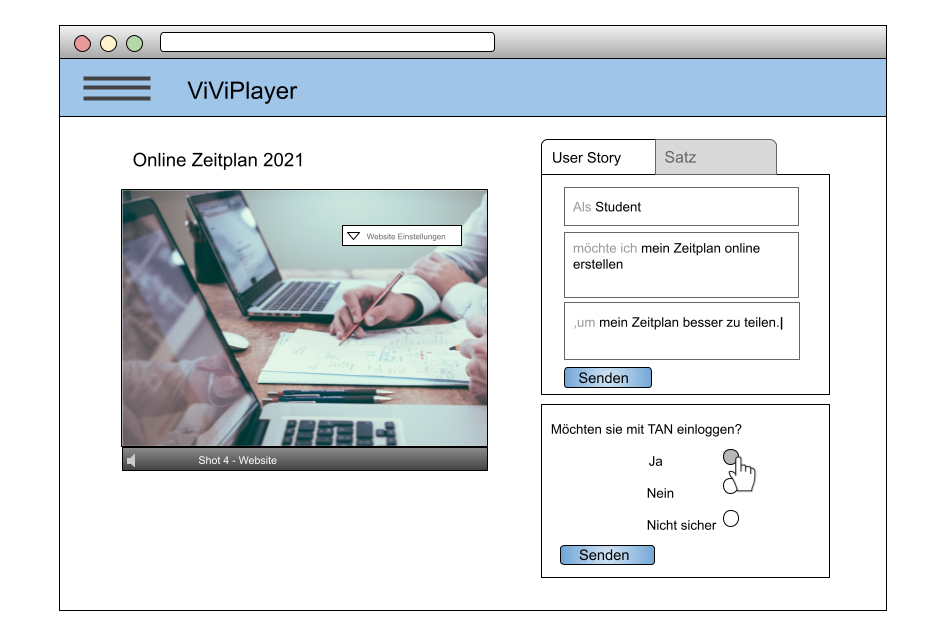
\includegraphics[width=\linewidth]{5dot1.png}
  \caption{Hier sieht man den ViViPlayer aus der Perspektive des Benutzers. Der Nutzer hat die Möglichkeit, strukturierte User-Stories oder Freitextsätze zu senden. Vom Moderator gestellte Fragen können direkt beantwortet werden. Der Videoplayer ermöglicht es dem Benutzer, das Video anzusehen, ohne die Wiedergabe für andere Teilnehmer zu stören. Vom Moderator bereitgestellte Annonatation können geöffnet und geschlossen werden.}
  \label{fig:5dot1}
\end{figure}

\begin{figure}
  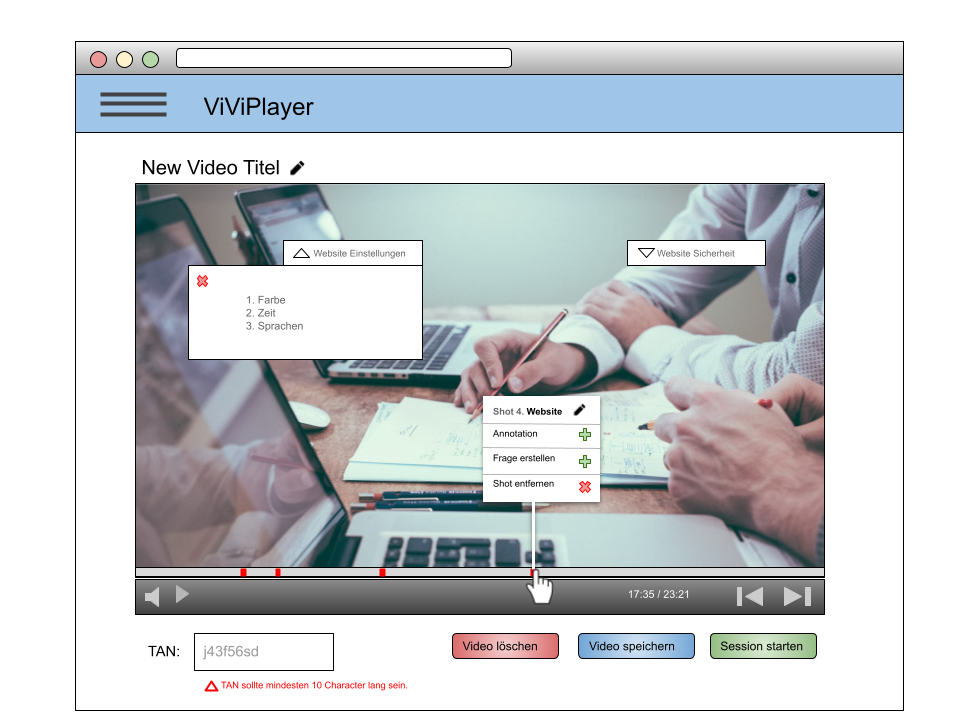
\includegraphics[width=\linewidth]{5dot2.png}
  \caption{Abbildung 2. Hier kann man sehen, wie ein neues Video für eine neue Sitzung von einem Moderator bearbeitet wird. Das Video wurde bereits automatisch in Kapitel unterteilt. Der Titel des Videos kann direkt geändert werden. Der Moderator hat die Möglichkeit, Kapitel und Annonatation hinzuzufügen und zu entfernen sowie jedem Kapitel Titel zuzuordnen und Fragen vorzuformulieren, indem er einfach auf die Segmente auf dem Video-Slider klickt. Wenn der Moderator mit dem Video zufrieden ist, kann er eine TAN vergeben und das Video entweder speichern oder direkt eine Live-Session starten.}
  \label{fig:5dot2}
\end{figure}

\begin{figure}
  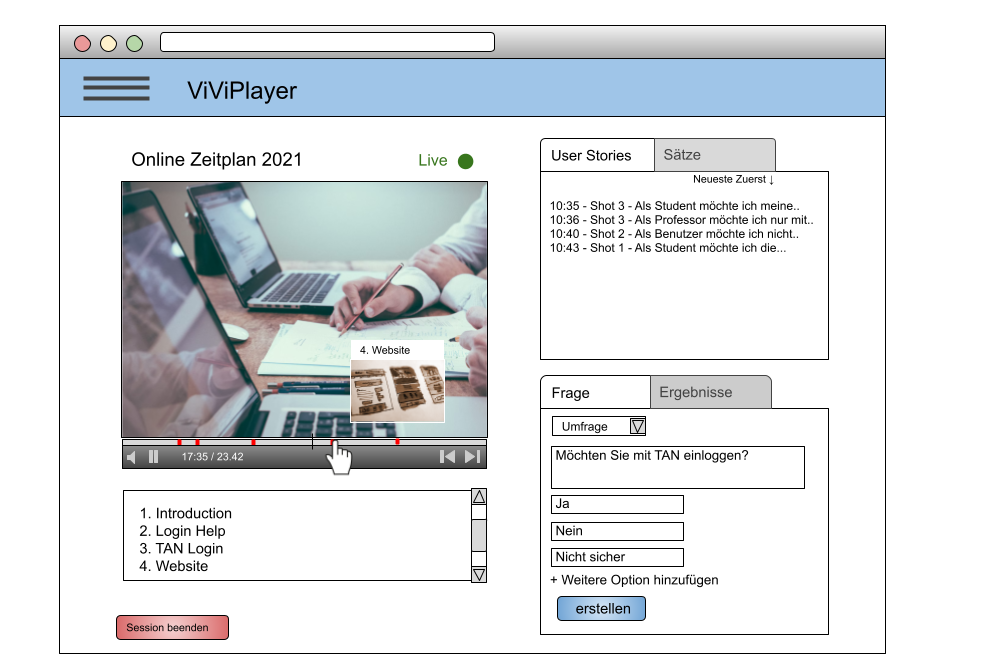
\includegraphics[width=\linewidth]{5dot3.png}
  \caption{Abbildung 3. Hier sieht man eine Live-Session aus der Sicht des Moderators. Im Gegensatz zur der Perspektive des Benutzers, hat der Moderator die volle Kontrolle über die Navigation des Videoplayers. Der Moderator hat die Möglichkeit, zu jedem gewünschten Teil des Videos zu springen. Zusätzliche Schaltflächen erleichtern es dem Moderator, zum Anfang oder Ende eines Kapitels zu springen. Der Moderator hat die Möglichkeit, Antworten von Benutzern zu lesen, sobald sie eintreffen. Dazu gehören User Stories, Sätze und Umfrageergebnisse.}
  \label{fig:5dot3}
\end{figure}


	\pagebreak
	\section{Probleme und Risiken}
\begin{enumerate}
	\item
    \textbf{WENN} es zu Verzögerungen im Projekt kommt \textbf{DANN} reicht die Zeit nicht aus, um nicht wesentliche Anforderungen zu entwickeln. Kunde wird am Ende unzufrieden sein.
    \linebreak
    \linebreak
    \textbf{Wahrscheinlichkeit:}  Da dieses Team zum ersten Mal zusammengearbeitet hat, ist es sehr schwer abzuschätzen, wie viel das Team in einem Sprint erreichen kann.
    \linebreak
    \linebreak
    \textbf{Abhilfe:} Das Team muss sich auf die obligatorischen Pflichtanforderungen konzentrieren, bevor es über zusätzliche Anforderungen nachdenkt.
    \linebreak

    \item
    \textbf{WENN} die Technologie mit dem bereitgestellten Produktionsserver nicht richtig funktioniert \textbf{DANN} sind Änderungen am Server und/oder der Software erforderlich, um die Kompatibilität zu gewährleisten. Dies kann später im Projektzyklus zu großen Verzögerungen führen.
    \linebreak
    \linebreak
    \textbf{Wahrscheinlichkeit:} Da der Server von der IT-Abteilung der Universität bereitgestellt wird und wir ein empfohlenes Framework (Django) verwenden, ist die Wahrscheinlichkeit einer Inkompatibilität gering.
    \linebreak
    \linebreak
    \textbf{Abhilfe:} Die Website sollte so früh wie möglich auf dem Produktionsserver getestet, um eventuelle Kompatibilitätsprobleme abzuschätzen.
    \linebreak
    
    \item
    \textbf{WENN} nur 1 Entwickler allein für den Kerncode verantwortlich ist \textbf{DANN} kann es zu Problemen kommen, wenn der Entwickler krankheits- oder aus anderen persönlichen Gründen arbeitsunfähig ist. Dies kann zu großen Verzögerungen im Projekt führen.
    \linebreak
    \linebreak
    \textbf{Wahrscheinlichkeit:} Es besteht immer die Möglichkeit, dass ein Entwickler seine Arbeit nicht fortsetzen kann.
    \linebreak
    \linebreak
    \textbf{Abhilfe:} Alle Entwickler sollten über ein funktionierendes Verständnis aller Aspekte des Quellcodes verfügen.
    \linebreak

    \item
    \textbf{WENN} es Verzögerungen bei der Synchronisierung von Videos gibt \textbf{DANN} können diese Verzögerungen dazu führen, dass sich Benutzer an einem falschen Ort befinden oder eine ruckartige Wiedergabe erleben.
    \linebreak
    \linebreak
    \textbf{Wahrscheinlichkeit:} Aufgrund normaler Schwankungen in der Verbindungsgeschwindigkeit und -verzögerung ist es sehr wahrscheinlich, dass Benutzer ein gewisses Maß an Synchronisierungsproblemen haben.
    \linebreak
    \linebreak
    \textbf{Abhilfe:}  Kleine Verzögerungen können ignoriert werden, um eine ruckelige Wiedergabe zu reduzieren. Die Videoqualität kann für Benutzer mit langsameren Verbindungen reduziert werden. Einschränkungen der Videogröße können implementiert werden.
    \linebreak
    
    \item
    \textbf{WENN} Benutzer einen inkompatiblen Browser verwenden \textbf{DANN} funktionieren möglicherweise bestimmte Funktionen nicht wie beabsichtigt.
    \linebreak
    \linebreak
    \textbf{Wahrscheinlichkeit:} Aufgrund der Vielzahl von Browsern, die unter anderem auf mobilen Geräten verwendet werden, ist es möglich, dass viele Browser nicht alle HTML 5-Standards oder -Funktionen unterstützen.
    \linebreak
    \linebreak
    \textbf{Abhilfe:} Die Website kann auf den gängigsten Webbrowsern der Welt getestet werden. Dies wird die Mehrheit der Benutzer abdecken. Außerdem können den Benutzern Browser-Empfehlungen präsentiert werden, um die Kompatibilität sicherzustellen.
    \linebreak


\end{enumerate}



	\pagebreak
	\section{Optionen zur Aufwandsreduktion}

	\subsection{Mögliche Abstriche}
	Die folgenden Funktionen der Web-App sind Sonderwünsche des Kunden, d.h. sie sind optionale Erweiterungen von der Web-App.
	\begin{itemize}
		\item Geschriebene Sätze werden automatisch vervollständigt.
		\item der Nutzer bekommt eine Rückmeldung für die geschriebenen Sätze anhand Anleitungen.
		\item Design Patterns für mögliche Erweiterungen, z.B. Android App fürs Schreiben der Anforderungen.
		\item Annotationen im Video.
	\end{itemize}
	
	\subsection{Inkrementelle Arbeit}
		\begin{enumerate}
			\item Iteration:
			\begin{itemize}
				\item Login für alle Benutzer.
				\item Video Segmentierung.
				\item TAN erstellen.
				\item User Story eingeben und posten.
				\item Session beenden.
				\item Registrierung für Moderator Rolle.
				\item Automatische Aufnahme des Video Frames für User Story.
				\item Automatisches Anhalten des Videos beim Wechseln zwischen den Shots.
			\end{itemize}
			\item Iteration:
			\begin{itemize}
				\item Anleitung für User Story.
				\item Umfragen stellen.
				\item Balkendiagramm für Ergebnis von Fragen.
				\item Text Navigation für Shots des ViVis.
				\item Session Daten exportieren von Server als .odt Datei.
				\item User Stories exportieren von Server als CSV Datei und Bilddatei.
				\item User Interface verbessern.
			\end{itemize}
			\item Optionale Erweiterungen:
			\begin{itemize}
				\item Video Annotation hinzufügen während des Abspielens.
				\item Automatisches Vervollständigen von Texteingaben.
				\item Automatische Rückmeldungen für geschriebene Anforderungen.
				\item API für Android oder iOS, z.B. fürs Schreiben von Anforderungen mit Handy.
			\end{itemize}
		\end{enumerate}


		
	\pagebreak
	\section{Glossar}

	\begin{description}
	\item{\textbf{ViVi}} Die Abkürzung für den Begriff "Vision Video".
	\end{description}

	\begin{description}
	\item{\textbf{Shot}} Ein Synonym für Segment oder Kapitel.
	\end{description}
	
	\begin{description}
	\item{\textbf{Session}} Ein Synonym für Sitzung zwischen den Teilnehmern.
	\end{description}

	\begin{description}
	\item{\textbf{Loadtest}} Testen des Systems durch Setzen einer Last, wie z. B. Datenbankanforderungen, um seine Leistung unter bestimmten Lasten zu ermitteln.
	\end{description}
	
	\begin{description}
    \item{\textbf{Walkthrough}} Jemand aus dem Entwicklungsteam beobachtet mit einem Teilnehmer die Nutzung der Software, um Feedback zu erhalten.
    \end{description}
    
    \begin{description}
    \item{\textbf{Black-Box-Test}} Tests basierend auf der Spezifikation ohne Einfluss des Quellcodes.
    \end{description}
    
    \begin{description}
    \item{\textbf{White-Box-Test}} Tests basierend auf reinen Merkmalen des Quellcodes wie z.B. 
    Funktionsparametern.
    \end{description}
    
    \begin{description}
    \item{\textbf{Penetrationstest}} Test um die Anfälligkeit für Angriffe zu ermitteln.
    \end{description}
    
    \begin{description}
    \item{\textbf{Teilnehmer}} Benutzer der an der Session teilnimmt ohne besondere Rechte.
    \end{description}
    
     \begin{description}
    \item{\textbf{Moderator}} Benutzer der an der Session teilnimmt mit besonderen Rechten. Dieser kann die Session verwalten und vorbereiten.
    \end{description}
    
    
 

	\pagebreak
	\section{Abnahme-Testfälle}
\begin{enumerate}
	\item \underline{\textbf{Testfall: UC 1 Moderator registrieren}} \linebreak
	\textbf{Setup:} Der Nutzer ist mit dem Internet verbunden und die Web-App ist geöffnet. Er befindet sich jetzt im Hauptmenü.\linebreak
	\textbf{Eingabe:} Der Nutzer klickt auf ''Registrieren.''.\linebreak
	\textbf{Ausgabe:} Der Nutzer wird zu Registrierungsseite weitergeleitet.\linebreak
	\textbf{Eingabe:} Der Nutzer gibt seine E-Mailadresse und ein Passwort und bestätigt dieses. Er klickt danach an ''Registrieren''. \linebreak
	\textbf{Ausgabe:} Die Daten sind zu einem Moderator weitergeleitet worden zum validieren.  Der Nutzer wird zum Hauptmenü weitergeleitet.
	
	\item \underline{\textbf{Testfall: UC 2 Moderator einloggen}} \linebreak
	\textbf{Setup:} Der Nutzer ist mit dem Internet verbunden und die Web-App ist geöffnet. Er befindet sich jetzt im Hauptmenü. \linebreak
	\textbf{Eingabe:} Der Nutzer klickt auf ''Einloggen als Moderator''. \linebreak
	\textbf{Ausgabe:} Ein Login Fenster taucht auf.\linebreak
	\textbf{Eingabe:} Der Nutzer hat keine Anmeldedaten eingegeben und klickt auf ''Anmelden''.\linebreak
	\textbf{Ausgabe:} Die Fehlermeldung ''Ungültige Anmeldedaten.'' erscheint unter dem Eingabefeld.
	
	\item \underline{\textbf{Testfall: UC 3 Teilnehmer einloggen}} \linebreak
	\textbf{Setup:} Der Nutzer ist mit dem Internet verbunden und die Web-App ist geöffnet. Er befindet sich jetzt im Hauptmenü. Eine ViViPlayer-Session ist von dem Moderator gestartet worden und im System ist die TAN 493489458 hinterlegt.
	Eine ViViPlayer-Session ist aber noch nicht von dem Moderator gestartet. \linebreak
	\textbf{Eingabe:} Der Nutzer klickt auf ''Einloggen als Teilnehmer'' an. \linebreak
	\textbf{Ausgabe:} Ein Login Fenster taucht auf.\linebreak
	\textbf{Eingabe:} Der Nutzer klickt auf ''Registrieren.'' an.\linebreak
	\textbf{Ausgabe:} Der Nutzer wird zu Registrierungsseite weitergeleitet.\linebreak
	\textbf{Eingabe:} Der Nutzer gibt seine E-mailadresse und ein Passwort und bestätigt dieses. Er klickt danach auf ''Registrieren'' an. \linebreak
	\textbf{Ausgabe:} Der Nutzer befindet sich jetzt in Validierungsvorgang. Die Validierung ist nicht erfolgreich. Nutzer ist gleich zurück zu Hauptmenü weitergeleitet und eine Nachricht ''Registrierung Fehlgeschlagen.'' wird gezeigt.\linebreak
	
	\item \underline{\textbf{Testfall}} \linebreak
	\textbf{Setup:} Der Nutzer ist mit dem Internet verbunden und öffnet die Web-App. Er befindet sich jetzt in Hauptmenü. Es gibt 2 Knöpfe, ''Session als Moderator starten'' und ''Session Teilnehmen''.
	Eine ViViPlayer-Session ist aber noch nicht von dem Moderator angefangen. \linebreak
	\textbf{Eingabe:} Der Nutzer klickt auf ''Session Teilnehmen.'' an. \linebreak
	\textbf{Ausgabe:} Ein Login Fenster taucht auf. Es gibt ein Eingabefeld für TAN.\linebreak
	\textbf{Eingabe:} Der Nutzer gibt eine 'falsche' TAN ein. \linebreak
	\textbf{Ausgabe:} Eine Fehlermeldung wird gezeigt.
	
	\item \underline{\textbf{Testfall: UC 3 Teilnehmer einloggen}} \linebreak
	\textbf{Setup:} Der Nutzer ist mit dem Internet verbunden und die Web-App ist geöffnet. Er befindet sich jetzt im Hauptmenü. Eine ViViPlayer-Session ist von dem Moderator gestartet worden und im System ist die TAN 493489458 hinterlegt. \linebreak
	\textbf{Eingabe:} Der Nutzer klickt auf ''Einloggen als Teilnehmer''. \linebreak
	\textbf{Ausgabe:} Ein Login Fenster taucht auf. .\linebreak
	\textbf{Eingabe:} Der Nutzer gibt die hinterlegte TAN ein. \linebreak
	\textbf{Ausgabe:} Der Nutzer bekommt eine Bestätigungsnachricht und er wird zu der ViViPlayer-Session weitergeleitet als Teilnehmer.

	\item \underline{\textbf{Testfall: UC 4 Session vorbereiten}} \linebreak
	\textbf{Setup:} Der Nutzer ist mit dem Internet verbunden und die Web-App ist geöffnet. Der Nutzer ist als Moderator angemeldet und befindet sich jetzt auf der Moderator-Hauptseite.\linebreak
	\textbf{Eingabe:} Der Nutzer klickt auf ''Session erstellen'' an.\linebreak
	\textbf{Ausgabe:} Das System zeigt die ViVi-Auswählen-Oberfläche an. \\
	\textbf{Eingabe:} Der Nutzer wählt ein ViVi und bestätigt(Testfall UC 5 ViVi auswählen).\\
	\textbf{Ausgabe:} Das System zeigt die ViVi-Segmentieren-Oberfläche an. \\
	\textbf{Eingabe:} Der Benutzer segmentiert das von ihm hochgeladene Video und bestätigt.(Testfall UC 6 ViVi Segmentieren)\\
	\textbf{Ausgabe:} Das System zeigt die Frage-Vorbereiten-Oberfläche an.\\
	\textbf{Eingabe:} Der Benutzer bereitet eine Um-/Verständnisfrage vor und bestätigt.(Testfall UC 7 Um-/Verständnisfragen erstellen)\\
	\textbf{Ausgabe:} Das System zeigt die ViVi-Überblick-Oberfläche an.\\
	\textbf{Eingabe:} Der Benutzer prüft noch mal alle Vorbereitungsschritte und klickt auf ''Erstellen''.\\
	\textbf{Ausgabe:} Das System erstellt eine neue Session und eine sichere TAN.
	
	\item \underline{\textbf{Testfall: UC 5 ViVi auswählen}} \linebreak
	\textbf{Setup:} Der Nutzer ist mit dem Internet verbunden und die Web-App ist geöffnet. Er ist als Moderator angemeldet. Der Benutzer ist im Vorgang, eine Session zu erstellen(Testfall UC 4 Session vorbereiten). Der Benutzer hat ein Vision Video in seinem Dateisystem gespeichert. \linebreak
	\textbf{Eingabe:} Der Nutzer klickt auf ''Hochladen''. \linebreak
	\textbf{Ausgabe:} Das System zeigt ein Fenster zum Hochladen des ViVis an.\\
	\textbf{Eingabe:} Der Nutzer wählt ein ViVi von seinem Dateisystem aus und bestätigt.\\
	\textbf{Ausgabe:} Das System zeigt die ViVi-Segmentieren-Oberfläche an.
	
	\item \underline{\textbf{Testfall: UC 6 ViVi segmentieren}} \linebreak
	\textbf{Setup:}Der Nutzer ist mit dem Internet verbunden und die Web-App ist geöffnet. Der Benutzer ist als Moderator angemeldet. Der Benutzer ist im Vorgang, eine Session zu erstellen(Testfall UC 4 Session vorbereiten). Der Benutzer hat ein Video ausgewählt. Der Benutzer befindet sich jetzt auf der ViVi-Segmentieren-Oberfläche.\linebreak
	\textbf{Eingabe:} Der Nutzer klickt auf den Video Slider, um einen bestimmten Shot auszuwählen. Er gibt den Titel für den Shot ein und klickt auf ''Hinzufügen''. \linebreak
	\textbf{Ausgabe:} Ein Zeitstempel für den ausgewählten Shot wird dem Slider hinzugefügt.\linebreak
	\textbf{Eingabe:} Der Nutzer klickt auf ''Weiter''. \linebreak
	\textbf{Ausgabe:} Der Nutzer wird zur nächsten Seite weitergeleitet. Eine Benutzeroberfläche für das Einfügen von Um-/Verständnisfragen wird gezeigt.
	
	\item \underline{\textbf{Testfall: UC 6 ViVi segmentieren}} \linebreak
	\textbf{Setup:} Der Nutzer ist mit dem Internet verbunden und die Web-App ist geöffnet. Der Benutzer ist als Moderator angemeldet. Der Benutzer ist im Vorgang, eine Session zu erstellen(Testfall UC 4 Session vorbereiten). Der Benutzer hat ein Video ausgewählt. Der Benutzer befindet sich jetzt auf der ViVi-Segmentieren-Oberfläche.\linebreak
	\textbf{Eingabe:} Der Nutzer klickt auf den Video Slider, um einen bestimmten Shot auszuwählen. Er gibt keinen Titel für den Shot ein und klickt auf ''Hinzufügen''. \linebreak
	\textbf{Ausgabe:} Eine Fehlermeldung wird gezeigt und kein neuer Shot wird hinzugefügt.
	
	\item \underline{\textbf{Testfall: UC 7 Um-/Verständnisfragen erstellen}} \linebreak
	\textbf{Setup:} Der Nutzer ist mit dem Internet verbunden und die Web-App ist geöffnet. Der Nutzer ist als Moderator angemeldet. Der Benutzer ist im Vorgang, eine Session zu erstellen(Testfall UC 4 Session vorbereiten). Der Nutzer hat ein Video ausgewählt und das Video in Shots segmentiert. Der Benutzer befindet sich jetzt auf der Frage-Vorbereiten-Oberfläche.\\
	\textbf{Eingabe:} Der Benutzer wählt den ''Um-/Verständnisfrage''-Modus aus. \\
	\textbf{Ausgabe:} Das System zeigt die Eingabe für Umfragen und Verständnisfragen an.\\ 
	\textbf{Eingabe:} Der Benutzer gibt keine Verständnisfrage an und bestätigt.\\
	\textbf{Ausgabe:} Das System gibt eine Fehlermeldung aus und die Umfrage oder Verständnisfrage wird weder angezeigt noch gespeichert.

	\item \underline{\textbf{Testfall: UC 8 ViVi navigieren}} \linebreak
	\textbf{Setup:} Der Nutzer ist mit dem Internet verbunden und die Web-App ist geöffnet. Der Nutzer ist als Moderator angemeldet. Eine ViViPlayer-Session ist von dem Nutzer gestartet worden(Testfall UC 4 Session vorbereiten). Ein weiterer Nutzer ist als Teilnehmer in der Session angemeldet. \\
	\textbf{Eingabe:} Der Benutzer bewegt den Slider an Stelle 01:40. \\
	\textbf{Ausgabe:} Das Video spielt an der Stelle 01:40 weiter für alle Teilnehmer.\\
	
	\item \underline{\textbf{Testfall: UC 9 Um-/Verständnisfragen in Session stellen}} \linebreak
	\textbf{Setup:} Der Nutzer ist mit dem Internet verbunden und die Web-App ist geöffnet. Der Nutzer ist als Moderator angemeldet. Es ist ein Video auf dem Server gespeichert. Der Nutzer hat ein Video ausgewählt und das Video in Shots segmentiert. Es gibt einen weiteren Teilnehmer, der angemeldet und Teil der Session ist.\\
	\textbf{Eingabe:} Der Benutzer wählt den ''Um-/Verständnisfrage''-Modus aus. \\
	\textbf{Ausgabe:} Das System zeigt die Eingabe für Umfragen und Verständnisfragen an.\\ 
	\textbf{Eingabe:} Der Benutzer gibt die Frage ''Kann ein Moderator eine User Story verfassen?'' und ein Zeitlimit von 60 Sekunden ein. Er legt fest, dass es sich um eine Verständnisfrage handelt und gibt die Antwortmöglichtkeiten ''Ja'' und ''Nein'' an. ''Ja'' wird als richtige Antwort festgelegt.\\
	\textbf{Ausgabe:} Das System zeigt die Frage allen Teilnehmern an.\\ 
	\textbf{Eingabe:} Alle Benutzer antworten auf die Umfrage innerhalb des Zeitlimits von 30 Sekunden.\\
	\textbf{Ausgabe:} Das System zeigt jedem Benutzer nach Ablauf des Zeitlimits das Ergebnis an. Die Verständnisfrage wird gespeichert und dem dazugehörigen Shot zugeordnet.\\
	
	\item \underline{\textbf{Testfall: UC 11 In Session kommentieren}} \linebreak
	\textbf{Setup:} Der Nutzer ist mit dem Internet verbunden und die Web-App ist geöffnet. Der Benutzer ist angemeldet und Teil der Session.\\
	\textbf{Eingabe:} Der Nutzer wählt den ''Kommentar''-Modus aus. \\
	\textbf{Ausgabe:} Das System zeigt die ''Kommentar''-Eingabe. \\
	\textbf{Eingabe:} Der Nutzer gibt ''Hello World'' ein und bestätigt wenn er fertig ist.\\
	\textbf{Ausgabe:} Das System verarbeitet die Anfrage und speichert den Kommentar ab. Die User Story wird den anderen Benutzern angezeigt und dem dazugehörigen Shot zugeordnet. \\
	
	\item \underline{\textbf{Testfall: UC 10 User-Story schreiben}} \linebreak
	\textbf{Setup:} Der Nutzer ist mit dem Internet verbunden und die Web-App ist geöffnet. Der Benutzer ist angemeldet und Teil der Session.\\
	\textbf{Eingabe:} Der Nutzer wählt den ''User Story''-Modus aus und gibt ''Damit ich weiß, ob jemand unregelmäßig arbeitet, möchte ich als Abteilungsleiter eine visuelle Darstellung der geleisteten Stunden sehen.'' und bestätigt wenn er fertig ist.\\
	\textbf{Ausgabe:} Das System verarbeitet die Anfrage und speichert die User Story ab. Die User Story wird den anderen Benutzern angezeigt und dem dazugehörigen Shot zugeordnet. \\
	
	\item \underline{\textbf{Testfall: UC 13 An Um-/Verständnisfragen teilnehmen}} \linebreak
	\textbf{Setup:} Der Nutzer ist mit dem Internet verbunden und die Web-App ist geöffnet. Der Nutzer ist als Teilnehmer angemeldet und Teil der Session. Der Nutzer befindet sich jetzt auf der ViViPlayer-Seite der Web-App. Der Moderator hat eine Um-/Verständnisfrage gestellt(Testfall UC 9 Um-/Verständnisfragen in Session stellen).\\
	\textbf{Eingabe:} Der Benutzer klickt auf eine Antwort der Um-/Verständnisfrage und auf ''Senden''.
	\textbf{Ausgabe:} Das System sammelt die Antworten von allen Benutzern und nach 30 Sekunden zeigt es diese in Form eines Balkendiagramms an.
	
	\item \underline{\textbf{Testfall: UC 12 Log-Dateien exportieren}} \linebreak
	\textbf{Setup:} Der Nutzer ist mit dem Internet verbunden und die Web-App ist geöffnet. Der Nutzer ist als Moderator angemeldet. Die ViViPlayer-Session ist von dem Nutzer beendet worden. Zusätzlich ist der Kommentar ''Hello World'', eine User Story ''Damit ich weiß, ob jemand unregelmäßig arbeitet, möchte ich als Abteilungsleiter eine visuelle Darstellung der geleisteten Stunden sehen.'' und die Verständnisfrage ''Kann der Moderator User Stories schreiben?'' mit den Antworten ''Ja'' und ''Nein'' auf dem Server gespeichert. Der Nutzer befindet sich jetzt auf der ViViPlayer-Seite. \\
	\textbf{Eingabe:} Der Benutzer klickt auf "Exportieren". \\
	\textbf{Ausgabe:} Das System erlaubt dem Benutzer alle Umfragen, Verständnisfragen, Shots mit Screenshots, Kommentare und User Stories in eine ''.odt''-Datei und die User Stories in eine ''.csv''-Datei zu exportieren und herunterzuladen.\\ 
	
\end{enumerate}


\end{document}

